\documentclass[xcolor=svgnames,9pt,english,aspectratio=169,t]{beamer}
%\documentclass[xcolor=svgnames,9pt,english,handout,aspectratio=169,t]{beamer}
\newcommand{\handout}{0}

% =====================================================================
% POLI 450A (2026) --- shared TEMPLATE layer.
%
% Input from each lecture near the top of its file, BEFORE
% ../course_theme.tex (metropolis must be selected before the course
% palette overrides it):
%
%   \documentclass[xcolor=svgnames,9pt,english,aspectratio=169]{beamer}
%   \newcommand{\handout}{0}
%   % =====================================================================
% POLI 450A (2026) --- shared TEMPLATE layer.
%
% Input from each lecture near the top of its file, BEFORE
% ../course_theme.tex (metropolis must be selected before the course
% palette overrides it):
%
%   \documentclass[xcolor=svgnames,9pt,english,aspectratio=169]{beamer}
%   \newcommand{\handout}{0}
%   % =====================================================================
% POLI 450A (2026) --- shared TEMPLATE layer.
%
% Input from each lecture near the top of its file, BEFORE
% ../course_theme.tex (metropolis must be selected before the course
% palette overrides it):
%
%   \documentclass[xcolor=svgnames,9pt,english,aspectratio=169]{beamer}
%   \newcommand{\handout}{0}
%   \input{../course_preamble.tex}
%   \input{../course_theme.tex}
%   \graphicspath{{./}{./figs/}}
%   \title[Short title]{450A Political Methodology I}
%   \subtitle{Lecture N: ...}
%
% Modeled on the 2026 Northwestern workshop template
% (Teaching/PanelData/_latex/2026/202608_Northwestern/workshop_preamble.tex).
%
% SCOPE: theme, beamer layout, packages, the roadmap hooks, and --- unlike
% the Northwestern decks --- the notation macros. The 450A lectures
% grew from one common ancestor, so their macro blocks agree wherever they
% overlap; merging them is safe. Three points where they had drifted are
% resolved here, and each is flagged inline below.
% =====================================================================

\usetheme{metropolis}
\metroset{sectionpage=none, subsectionpage=none, numbering=none}
\setbeamertemplate{navigation symbols}{}

\setbeamersize{text margin left=5mm, text margin right=5mm}
\setbeamertemplate{itemize/enumerate body begin}{\leftmargini=1.5em\relax}
\setbeamertemplate{itemize/enumerate subbody begin}{\leftmarginii=1.5em\relax}
\setbeamertemplate{itemize/enumerate subsubbody begin}{\leftmarginiii=1.5em\relax}

% ----------------------------------------------------------- top alignment
% Every deck passes the t class option, so beamer applies the frame key
% below to every frame (explicit [plain,c] frames — title page, roadmaps —
% stay centered). Beamer's stock t key puts a rigid .2cm pad above the
% content; frames sized to this template's full-height ceilings then run
% Overfull \vbox by up to that pad. Same key as beamerbaseframe.sty, with
% one change: the pad may shrink to zero when the frame is full.
\makeatletter
\define@key{beamerframe}{t}[true]{% top
  \beamer@frametopskip=.2cm plus .5\paperheight minus .2cm\relax%
  \beamer@framebottomskip=0pt plus 1fill\relax%
  \beamer@frametopskipautobreak=\beamer@frametopskip\relax%
  \beamer@framebottomskipautobreak=\beamer@framebottomskip\relax%
}

% ------------------------------------------------- slide-top check (2026-10-11)
% A slide whose content is too tall for the frame is squeezed: the pad above
% shrinks and its content starts higher than on other slides, so a figure
% "wobbles" when the class steps from one slide to the next (Lecture 4-1,
% slides 1-2, 2026-10-11). The marker below records where each slide's
% content starts (a whatsit: it adds no space and moves nothing).
% `python3 ../check_slides.py lec<N>` then lists every slide that starts
% higher than the deck's normal position. That list must be empty.
% Recorded per slide: page, frame number, content-top y (sp), the room left
% below the title bar, and P for a plain frame (title page, roadmaps).
\providecommand\slidetop[5]{}
\AtBeginDocument{\immediate\write\@auxout{\string\providecommand\string\slidetop[5]{}}}
\def\beamer@markframetop{%
  \pdfsavepos
  \edef\beamer@marktmp{\noexpand\write\noexpand\@auxout{\string\slidetop
    {\noexpand\thepage}{\noexpand\insertframenumber}{\noexpand\the\noexpand\pdflastypos}%
    {\number\beamer@frametextheight}{\ifbeamer@plainframe P\else N\fi}}}%
  \beamer@marktmp}
\RequirePackage{etoolbox}
\patchcmd{\endbeamer@frameslide}
  {\vskip\beamer@frametopskip}
  {\vskip\beamer@frametopskip\beamer@markframetop}
  {}{\PackageWarning{course_preamble}{slide-top marker not installed}}
\makeatother

% ---------------------------------------------------------------- packages
\usepackage{xcolor}
\usepackage{colortbl}
\usepackage{amsmath}
\usepackage{amsfonts}
\usepackage{amssymb}
\usepackage{bm}
\usepackage{graphicx}
\usepackage{multirow}
\usepackage{fancyvrb}
\usepackage{listings}
\usepackage{tikz}
\usetikzlibrary{arrows.meta,positioning,decorations.pathreplacing}

% --------------------------------------------------------- figure fitting
% Default bounding box for every \includegraphics that does not override it.
% With keepaspectratio the image is scaled to fit *inside* width x height, so
% a figure can never run past the side margins or off the bottom of a slide.
% Options given at the call site override these on a per-key basis: e.g.
% [width=.6\linewidth] narrows the box but keeps the height ceiling.
% \figmaxheight is set at \begin{document}: beamer only computes the final
% \textheight once the head/foot templates are known. 0.80 is just under what a
% frame with a title and one line of text can hold (measured: 0.834\textheight);
% a frame that needs more room for text can lower it locally.
\newlength{\figmaxheight}
\AtBeginDocument{\setlength{\figmaxheight}{0.80\textheight}}
\setkeys{Gin}{width=\linewidth,height=\figmaxheight,keepaspectratio}

% -------------------------------------------------------- roadmap frames
% Identical in all lectures. A lecture that does not want the
% subsection roadmap clears it after the \input with \AtBeginSubsection[]{}.
% hideothersubsections is load-bearing, not cosmetic: lecture 4 had 13
% subsections before it was split into 4-1, 4-2 and 4-3 (2026-10-09), and a
% full contents list ran off the top and bottom of the slide. Hiding the other sections' subsections caps the list at 10 lines.
\subject{Talks}
% No back-to-back roadmaps (Yiqing, 2026-10-11): when a subsection starts right
% after its section's roadmap, with no content slide in between, its own
% roadmap would repeat the one just shown (5-1's handout showed "Two Cases"
% twice), so it is skipped. The section roadmap records the frame count; the
% subsection roadmap appears only if a content slide has come since.
\makeatletter
\def\course@secframe{-1}
\AtBeginSection[]
{
  \begin{frame}[plain,c]
    \frametitle{}
    \tableofcontents[currentsection,hideothersubsections]
    \addtocounter{framenumber}{-1}
  \end{frame}
  \xdef\course@secframe{\the\c@framenumber}
}
\AtBeginSubsection[]
{
  \ifnum\c@framenumber=\course@secframe\relax\else
  \begin{frame}[plain,c]
    \frametitle{}
    \tableofcontents[currentsection,currentsubsection,hideothersubsections]
    \addtocounter{framenumber}{-1}
  \end{frame}
  \fi
}
\makeatother

% ------------------------------------------------------ theorem environments
\newtheorem{assumption}{Assumption}
\newtheorem{iass}{Identification Assumption}
\newtheorem{ires}{Identification Result}
\newtheorem{estm}{Estimand}
\newtheorem{esti}{Estimator}
\newtheorem{question}{Question}
\newtheorem{answer}{Answer}
\newtheorem{proposition}{Proposition}

% =====================================================================
% Notation
% =====================================================================
\definecolor{dgreen}{rgb}{0,.6,0.8}

\renewcommand\r{\right}
\renewcommand\l{\left}
\newcommand{\bs}{\boldsymbol}
\newcommand{\mb}{\mathbf}
\newcommand{\real}{\mathbb{R}}
\newcommand{\cN}{\mathcal{N}}
\newcommand{\E}{\mathbb{E}}
\newcommand{\V}{\mathbb{V}}

% MERGE NOTE 1. Lecture 2-4 set \epsilon to \varepsilon; the other twelve
% left it at the upright default. Adopting \varepsilon course-wide so the
% error term looks the same in every lecture.
\renewcommand{\epsilon}{\varepsilon}

% MERGE NOTE 2. Lecture 2-4 wrote its vectors as \bm (bold italic); the other
% twelve use \mathbf (bold upright). \mathbf wins --- it is the convention in
% eleven of the thirteen decks and in the course's matrix lectures. Only
% \iid, \E, \cN and \Var from that block are actually used in 2-4's body.
\renewcommand{\u}{\ensuremath{\mb{u}}}
\renewcommand{\v}{\ensuremath{\mb{v}}}
\newcommand{\U}{\ensuremath{\mb{U}}}
\newcommand{\M}{\ensuremath{\mb{M}}}
\newcommand{\X}{\ensuremath{\mb{X}}}
\newcommand{\x}{\ensuremath{\mb{x}}}
\newcommand{\y}{\ensuremath{\mb{y}}}
\newcommand{\Z}{\ensuremath{\mb{Z}}}
\newcommand{\C}{\ensuremath{\mb{C}}}
\newcommand{\D}{\ensuremath{\mb{D}}}
\newcommand{\I}{\ensuremath{\mb{I}}}
\newcommand{\W}{\ensuremath{\mb{W}}}
\renewcommand{\a}{\ensuremath{\mb{a}}}
\renewcommand{\P}{\ensuremath{\mb{P}}}
\newcommand{\one}{\ensuremath{\mb{1}}}
\newcommand{\zero}{\ensuremath{\mb{0}}}

\renewcommand{\b}{\ensuremath{\bs{\beta}}}
\newcommand{\be}{\ensuremath{\bs{\beta}}}
\newcommand{\e}{\ensuremath{\bs{\epsilon}}}
\newcommand{\eps}{\ensuremath{\bs{\epsilon}}}
\newcommand{\eeta}{\ensuremath{\bs{\eta}}}
\newcommand{\bhat}{\ensuremath{\hat{\bs{\beta}}}}
\newcommand{\ehat}{\ensuremath{\hat{\e}}}
\newcommand{\Sig}{\ensuremath{\bs{\Sigma}}}
\newcommand{\SigInv}{\ensuremath{\bs{\Sigma^{-1}}}}

\newcommand{\XX}{\ensuremath{\X'\X}}
\newcommand{\XXinv}{\ensuremath{\left(\XX\right)^{-1}}}
\newcommand{\hatmat}{\ensuremath{\X \XXinv \X'}}
\newcommand{\hatsig}{\ensuremath{\hat{\sigma}^2}}
\newcommand{\sig}{\ensuremath{\sigma^2}}

\newcommand{\cA}{\mathcal{A}}
\newcommand{\cJ}{\mathcal{J}}
\newcommand{\cL}{\mathcal{L}}
\newcommand{\cLL}{\mathcal{LL}}
\newcommand{\cll}{\ell}
\newcommand{\cQ}{\mathcal{Q}}
\newcommand{\cP}{\mathcal{P}}

% MERGE NOTE 3. \var / \Var and \cov / \Cov were spelled with \text in some
% lectures and \mbox in others. Same output; \text kept.
\newcommand{\var}{\text{Var}}
\newcommand{\Var}{\text{Var}}
\newcommand{\cov}{\text{Cov}}
\newcommand{\Cov}{\text{Cov}}
\newcommand{\cor}{\text{Cor}}
\newcommand{\tr}{\text{tr}}
\newcommand{\avepop}{\frac{1}{n}\sum_{i=1}^n}

\DeclareMathOperator*\plim{plim}
\DeclareMathOperator\rank{rank}
\DeclareMathOperator*\argmax{argmax}
\DeclareMathOperator*\argmin{argmin}
\DeclareMathOperator{\sgn}{sgn}
\newcommand{\diag}{\mathop{\mathrm{diag}}}

\newcommand\ud{\mathrm{d}}
\newcommand\dist{\buildrel\rm d\over\sim}
\newcommand\ind{\stackrel{\rm indep.}{\sim}}
\newcommand\iid{\stackrel{\rm i.i.d.}{\sim}}
\newcommand\logit{{\rm logit}}

\newcommand\indep{\protect\mathpalette{\protect\independenT}{\perp}}
\def\independenT#1#2{\mathrel{\rlap{$#1#2$}\mkern2mu{#1#2}}}

% ------------------------------------------------------------- text helpers
\newcommand{\bi}{\begin{itemize}}
\newcommand{\ei}{\end{itemize}}
\newcommand{\noi}{\noindent}
\newcommand{\red}{\textcolor{Cardinal}}
\newcommand{\blue}{\textcolor{CourseBlue}}
\newcommand{\gray}{\textcolor{gray}}
\newcommand\spacingset[1]{\renewcommand{\baselinestretch}{#1}\small\normalsize}

\hyphenation{tyamamot}


% ------------------------------------------------ figure-position check (2026-10-11)
% Records where every \includegraphics lands and its size (a whatsit; it moves
% nothing). check_slides.py flags two consecutive slides that show a figure of
% the same size in different places: the class sees it jump (Lecture 3, slides
% 18 to 19: one frame had \vspace{.3cm} above the figure, the next did not),
% and two consecutive slides that show the same file at different sizes or
% places (Lecture 6-3, slides 10 to 11, the ballot image). The file name is the
% seventh field.
\makeatletter
\providecommand\figpos[7]{}
\AtBeginDocument{\immediate\write\@auxout{\string\providecommand\string\figpos[7]{}}}
\newbox\course@figbox
\let\course@origGinclude\Ginclude@graphics
\def\Ginclude@graphics#1{%
  \setbox\course@figbox\hbox{\course@origGinclude{#1}}%
  \pdfsavepos
  \edef\course@figtmp{\noexpand\write\noexpand\@auxout{\string\figpos
    {\noexpand\thepage}{\noexpand\insertframenumber}%
    {\noexpand\the\noexpand\pdflastxpos}{\noexpand\the\noexpand\pdflastypos}%
    {\number\wd\course@figbox}{\number\ht\course@figbox}{\detokenize{#1}}}}%
  \course@figtmp
  \box\course@figbox}
\makeatother

%   % =====================================================================
% POLI 450A (2026) --- shared visual system.
% Input from each lecture AFTER ../course_preamble.tex.
%
% Same shape as the 2026 Northwestern workshop theme
% (Teaching/PanelData/_latex/2026/202608_Northwestern/workshop_theme.tex),
% with the workshop's purple swapped for the course's cardinal. Kept
% deliberately light so the lecture sources stay easy to edit.
%
% To retune the course to Stanford's official cardinal, change the one
% Cardinal line below to HTML 8C1515.
% =====================================================================
\definecolor{Cardinal}{HTML}{A8003B}     % primary: titles, structure, alerts
\definecolor{CourseInk}{HTML}{252A34}    % body text
\definecolor{CourseBlue}{HTML}{2F6B9A}   % secondary accent
\definecolor{CourseMist}{HTML}{F8F1F4}   % block backgrounds

\setbeamercolor{normal text}{fg=CourseInk,bg=white}
\setbeamercolor{structure}{fg=Cardinal}
\setbeamercolor{alerted text}{fg=Cardinal}
\setbeamercolor{frametitle}{fg=white,bg=Cardinal}
\setbeamercolor{title}{fg=Cardinal}
\setbeamercolor{subtitle}{fg=CourseInk}
\setbeamercolor{block title}{fg=white,bg=Cardinal}
\setbeamercolor{block body}{fg=CourseInk,bg=CourseMist}
\setbeamercolor{section in toc}{fg=Cardinal}
\setbeamercolor{subsection in toc}{fg=CourseInk}
\setbeamercolor{itemize item}{fg=Cardinal}
\setbeamercolor{itemize subitem}{fg=Cardinal}
\setbeamercolor{enumerate item}{fg=Cardinal}

\setbeamerfont{title}{series=\bfseries,size=\Large}
\setbeamerfont{frametitle}{series=\bfseries,size=\large}
\setbeamerfont{block title}{series=\bfseries}
\setbeamertemplate{navigation symbols}{}
\setbeamertemplate{items}[circle]
\setbeamertemplate{blocks}[rounded][shadow=false]
\setbeamertemplate{frametitle continuation}{}
\setbeamertemplate{footline}{%
  \leavevmode\hbox{%
  \begin{beamercolorbox}[wd=.88\paperwidth,ht=2.6ex,dp=1.2ex,leftskip=1.2em]{author in head/foot}%
  \usebeamerfont{author in head/foot}\insertshorttitle
  \end{beamercolorbox}%
  \begin{beamercolorbox}[wd=.12\paperwidth,ht=2.6ex,dp=1.2ex,center]{date in head/foot}%
  \insertframenumber
  \end{beamercolorbox}}}

\newcommand{\slidesource}[1]{\vfill{\scriptsize\color{gray}Source: #1}}
\newcommand{\keyquestion}[1]{\begin{block}{Question}#1\end{block}}

%   \graphicspath{{./}{./figs/}}
%   \title[Short title]{450A Political Methodology I}
%   \subtitle{Lecture N: ...}
%
% Modeled on the 2026 Northwestern workshop template
% (Teaching/PanelData/_latex/2026/202608_Northwestern/workshop_preamble.tex).
%
% SCOPE: theme, beamer layout, packages, the roadmap hooks, and --- unlike
% the Northwestern decks --- the notation macros. The 450A lectures
% grew from one common ancestor, so their macro blocks agree wherever they
% overlap; merging them is safe. Three points where they had drifted are
% resolved here, and each is flagged inline below.
% =====================================================================

\usetheme{metropolis}
\metroset{sectionpage=none, subsectionpage=none, numbering=none}
\setbeamertemplate{navigation symbols}{}

\setbeamersize{text margin left=5mm, text margin right=5mm}
\setbeamertemplate{itemize/enumerate body begin}{\leftmargini=1.5em\relax}
\setbeamertemplate{itemize/enumerate subbody begin}{\leftmarginii=1.5em\relax}
\setbeamertemplate{itemize/enumerate subsubbody begin}{\leftmarginiii=1.5em\relax}

% ----------------------------------------------------------- top alignment
% Every deck passes the t class option, so beamer applies the frame key
% below to every frame (explicit [plain,c] frames — title page, roadmaps —
% stay centered). Beamer's stock t key puts a rigid .2cm pad above the
% content; frames sized to this template's full-height ceilings then run
% Overfull \vbox by up to that pad. Same key as beamerbaseframe.sty, with
% one change: the pad may shrink to zero when the frame is full.
\makeatletter
\define@key{beamerframe}{t}[true]{% top
  \beamer@frametopskip=.2cm plus .5\paperheight minus .2cm\relax%
  \beamer@framebottomskip=0pt plus 1fill\relax%
  \beamer@frametopskipautobreak=\beamer@frametopskip\relax%
  \beamer@framebottomskipautobreak=\beamer@framebottomskip\relax%
}

% ------------------------------------------------- slide-top check (2026-10-11)
% A slide whose content is too tall for the frame is squeezed: the pad above
% shrinks and its content starts higher than on other slides, so a figure
% "wobbles" when the class steps from one slide to the next (Lecture 4-1,
% slides 1-2, 2026-10-11). The marker below records where each slide's
% content starts (a whatsit: it adds no space and moves nothing).
% `python3 ../check_slides.py lec<N>` then lists every slide that starts
% higher than the deck's normal position. That list must be empty.
% Recorded per slide: page, frame number, content-top y (sp), the room left
% below the title bar, and P for a plain frame (title page, roadmaps).
\providecommand\slidetop[5]{}
\AtBeginDocument{\immediate\write\@auxout{\string\providecommand\string\slidetop[5]{}}}
\def\beamer@markframetop{%
  \pdfsavepos
  \edef\beamer@marktmp{\noexpand\write\noexpand\@auxout{\string\slidetop
    {\noexpand\thepage}{\noexpand\insertframenumber}{\noexpand\the\noexpand\pdflastypos}%
    {\number\beamer@frametextheight}{\ifbeamer@plainframe P\else N\fi}}}%
  \beamer@marktmp}
\RequirePackage{etoolbox}
\patchcmd{\endbeamer@frameslide}
  {\vskip\beamer@frametopskip}
  {\vskip\beamer@frametopskip\beamer@markframetop}
  {}{\PackageWarning{course_preamble}{slide-top marker not installed}}
\makeatother

% ---------------------------------------------------------------- packages
\usepackage{xcolor}
\usepackage{colortbl}
\usepackage{amsmath}
\usepackage{amsfonts}
\usepackage{amssymb}
\usepackage{bm}
\usepackage{graphicx}
\usepackage{multirow}
\usepackage{fancyvrb}
\usepackage{listings}
\usepackage{tikz}
\usetikzlibrary{arrows.meta,positioning,decorations.pathreplacing}

% --------------------------------------------------------- figure fitting
% Default bounding box for every \includegraphics that does not override it.
% With keepaspectratio the image is scaled to fit *inside* width x height, so
% a figure can never run past the side margins or off the bottom of a slide.
% Options given at the call site override these on a per-key basis: e.g.
% [width=.6\linewidth] narrows the box but keeps the height ceiling.
% \figmaxheight is set at \begin{document}: beamer only computes the final
% \textheight once the head/foot templates are known. 0.80 is just under what a
% frame with a title and one line of text can hold (measured: 0.834\textheight);
% a frame that needs more room for text can lower it locally.
\newlength{\figmaxheight}
\AtBeginDocument{\setlength{\figmaxheight}{0.80\textheight}}
\setkeys{Gin}{width=\linewidth,height=\figmaxheight,keepaspectratio}

% -------------------------------------------------------- roadmap frames
% Identical in all lectures. A lecture that does not want the
% subsection roadmap clears it after the \input with \AtBeginSubsection[]{}.
% hideothersubsections is load-bearing, not cosmetic: lecture 4 had 13
% subsections before it was split into 4-1, 4-2 and 4-3 (2026-10-09), and a
% full contents list ran off the top and bottom of the slide. Hiding the other sections' subsections caps the list at 10 lines.
\subject{Talks}
% No back-to-back roadmaps (Yiqing, 2026-10-11): when a subsection starts right
% after its section's roadmap, with no content slide in between, its own
% roadmap would repeat the one just shown (5-1's handout showed "Two Cases"
% twice), so it is skipped. The section roadmap records the frame count; the
% subsection roadmap appears only if a content slide has come since.
\makeatletter
\def\course@secframe{-1}
\AtBeginSection[]
{
  \begin{frame}[plain,c]
    \frametitle{}
    \tableofcontents[currentsection,hideothersubsections]
    \addtocounter{framenumber}{-1}
  \end{frame}
  \xdef\course@secframe{\the\c@framenumber}
}
\AtBeginSubsection[]
{
  \ifnum\c@framenumber=\course@secframe\relax\else
  \begin{frame}[plain,c]
    \frametitle{}
    \tableofcontents[currentsection,currentsubsection,hideothersubsections]
    \addtocounter{framenumber}{-1}
  \end{frame}
  \fi
}
\makeatother

% ------------------------------------------------------ theorem environments
\newtheorem{assumption}{Assumption}
\newtheorem{iass}{Identification Assumption}
\newtheorem{ires}{Identification Result}
\newtheorem{estm}{Estimand}
\newtheorem{esti}{Estimator}
\newtheorem{question}{Question}
\newtheorem{answer}{Answer}
\newtheorem{proposition}{Proposition}

% =====================================================================
% Notation
% =====================================================================
\definecolor{dgreen}{rgb}{0,.6,0.8}

\renewcommand\r{\right}
\renewcommand\l{\left}
\newcommand{\bs}{\boldsymbol}
\newcommand{\mb}{\mathbf}
\newcommand{\real}{\mathbb{R}}
\newcommand{\cN}{\mathcal{N}}
\newcommand{\E}{\mathbb{E}}
\newcommand{\V}{\mathbb{V}}

% MERGE NOTE 1. Lecture 2-4 set \epsilon to \varepsilon; the other twelve
% left it at the upright default. Adopting \varepsilon course-wide so the
% error term looks the same in every lecture.
\renewcommand{\epsilon}{\varepsilon}

% MERGE NOTE 2. Lecture 2-4 wrote its vectors as \bm (bold italic); the other
% twelve use \mathbf (bold upright). \mathbf wins --- it is the convention in
% eleven of the thirteen decks and in the course's matrix lectures. Only
% \iid, \E, \cN and \Var from that block are actually used in 2-4's body.
\renewcommand{\u}{\ensuremath{\mb{u}}}
\renewcommand{\v}{\ensuremath{\mb{v}}}
\newcommand{\U}{\ensuremath{\mb{U}}}
\newcommand{\M}{\ensuremath{\mb{M}}}
\newcommand{\X}{\ensuremath{\mb{X}}}
\newcommand{\x}{\ensuremath{\mb{x}}}
\newcommand{\y}{\ensuremath{\mb{y}}}
\newcommand{\Z}{\ensuremath{\mb{Z}}}
\newcommand{\C}{\ensuremath{\mb{C}}}
\newcommand{\D}{\ensuremath{\mb{D}}}
\newcommand{\I}{\ensuremath{\mb{I}}}
\newcommand{\W}{\ensuremath{\mb{W}}}
\renewcommand{\a}{\ensuremath{\mb{a}}}
\renewcommand{\P}{\ensuremath{\mb{P}}}
\newcommand{\one}{\ensuremath{\mb{1}}}
\newcommand{\zero}{\ensuremath{\mb{0}}}

\renewcommand{\b}{\ensuremath{\bs{\beta}}}
\newcommand{\be}{\ensuremath{\bs{\beta}}}
\newcommand{\e}{\ensuremath{\bs{\epsilon}}}
\newcommand{\eps}{\ensuremath{\bs{\epsilon}}}
\newcommand{\eeta}{\ensuremath{\bs{\eta}}}
\newcommand{\bhat}{\ensuremath{\hat{\bs{\beta}}}}
\newcommand{\ehat}{\ensuremath{\hat{\e}}}
\newcommand{\Sig}{\ensuremath{\bs{\Sigma}}}
\newcommand{\SigInv}{\ensuremath{\bs{\Sigma^{-1}}}}

\newcommand{\XX}{\ensuremath{\X'\X}}
\newcommand{\XXinv}{\ensuremath{\left(\XX\right)^{-1}}}
\newcommand{\hatmat}{\ensuremath{\X \XXinv \X'}}
\newcommand{\hatsig}{\ensuremath{\hat{\sigma}^2}}
\newcommand{\sig}{\ensuremath{\sigma^2}}

\newcommand{\cA}{\mathcal{A}}
\newcommand{\cJ}{\mathcal{J}}
\newcommand{\cL}{\mathcal{L}}
\newcommand{\cLL}{\mathcal{LL}}
\newcommand{\cll}{\ell}
\newcommand{\cQ}{\mathcal{Q}}
\newcommand{\cP}{\mathcal{P}}

% MERGE NOTE 3. \var / \Var and \cov / \Cov were spelled with \text in some
% lectures and \mbox in others. Same output; \text kept.
\newcommand{\var}{\text{Var}}
\newcommand{\Var}{\text{Var}}
\newcommand{\cov}{\text{Cov}}
\newcommand{\Cov}{\text{Cov}}
\newcommand{\cor}{\text{Cor}}
\newcommand{\tr}{\text{tr}}
\newcommand{\avepop}{\frac{1}{n}\sum_{i=1}^n}

\DeclareMathOperator*\plim{plim}
\DeclareMathOperator\rank{rank}
\DeclareMathOperator*\argmax{argmax}
\DeclareMathOperator*\argmin{argmin}
\DeclareMathOperator{\sgn}{sgn}
\newcommand{\diag}{\mathop{\mathrm{diag}}}

\newcommand\ud{\mathrm{d}}
\newcommand\dist{\buildrel\rm d\over\sim}
\newcommand\ind{\stackrel{\rm indep.}{\sim}}
\newcommand\iid{\stackrel{\rm i.i.d.}{\sim}}
\newcommand\logit{{\rm logit}}

\newcommand\indep{\protect\mathpalette{\protect\independenT}{\perp}}
\def\independenT#1#2{\mathrel{\rlap{$#1#2$}\mkern2mu{#1#2}}}

% ------------------------------------------------------------- text helpers
\newcommand{\bi}{\begin{itemize}}
\newcommand{\ei}{\end{itemize}}
\newcommand{\noi}{\noindent}
\newcommand{\red}{\textcolor{Cardinal}}
\newcommand{\blue}{\textcolor{CourseBlue}}
\newcommand{\gray}{\textcolor{gray}}
\newcommand\spacingset[1]{\renewcommand{\baselinestretch}{#1}\small\normalsize}

\hyphenation{tyamamot}


% ------------------------------------------------ figure-position check (2026-10-11)
% Records where every \includegraphics lands and its size (a whatsit; it moves
% nothing). check_slides.py flags two consecutive slides that show a figure of
% the same size in different places: the class sees it jump (Lecture 3, slides
% 18 to 19: one frame had \vspace{.3cm} above the figure, the next did not),
% and two consecutive slides that show the same file at different sizes or
% places (Lecture 6-3, slides 10 to 11, the ballot image). The file name is the
% seventh field.
\makeatletter
\providecommand\figpos[7]{}
\AtBeginDocument{\immediate\write\@auxout{\string\providecommand\string\figpos[7]{}}}
\newbox\course@figbox
\let\course@origGinclude\Ginclude@graphics
\def\Ginclude@graphics#1{%
  \setbox\course@figbox\hbox{\course@origGinclude{#1}}%
  \pdfsavepos
  \edef\course@figtmp{\noexpand\write\noexpand\@auxout{\string\figpos
    {\noexpand\thepage}{\noexpand\insertframenumber}%
    {\noexpand\the\noexpand\pdflastxpos}{\noexpand\the\noexpand\pdflastypos}%
    {\number\wd\course@figbox}{\number\ht\course@figbox}{\detokenize{#1}}}}%
  \course@figtmp
  \box\course@figbox}
\makeatother

%   % =====================================================================
% POLI 450A (2026) --- shared visual system.
% Input from each lecture AFTER ../course_preamble.tex.
%
% Same shape as the 2026 Northwestern workshop theme
% (Teaching/PanelData/_latex/2026/202608_Northwestern/workshop_theme.tex),
% with the workshop's purple swapped for the course's cardinal. Kept
% deliberately light so the lecture sources stay easy to edit.
%
% To retune the course to Stanford's official cardinal, change the one
% Cardinal line below to HTML 8C1515.
% =====================================================================
\definecolor{Cardinal}{HTML}{A8003B}     % primary: titles, structure, alerts
\definecolor{CourseInk}{HTML}{252A34}    % body text
\definecolor{CourseBlue}{HTML}{2F6B9A}   % secondary accent
\definecolor{CourseMist}{HTML}{F8F1F4}   % block backgrounds

\setbeamercolor{normal text}{fg=CourseInk,bg=white}
\setbeamercolor{structure}{fg=Cardinal}
\setbeamercolor{alerted text}{fg=Cardinal}
\setbeamercolor{frametitle}{fg=white,bg=Cardinal}
\setbeamercolor{title}{fg=Cardinal}
\setbeamercolor{subtitle}{fg=CourseInk}
\setbeamercolor{block title}{fg=white,bg=Cardinal}
\setbeamercolor{block body}{fg=CourseInk,bg=CourseMist}
\setbeamercolor{section in toc}{fg=Cardinal}
\setbeamercolor{subsection in toc}{fg=CourseInk}
\setbeamercolor{itemize item}{fg=Cardinal}
\setbeamercolor{itemize subitem}{fg=Cardinal}
\setbeamercolor{enumerate item}{fg=Cardinal}

\setbeamerfont{title}{series=\bfseries,size=\Large}
\setbeamerfont{frametitle}{series=\bfseries,size=\large}
\setbeamerfont{block title}{series=\bfseries}
\setbeamertemplate{navigation symbols}{}
\setbeamertemplate{items}[circle]
\setbeamertemplate{blocks}[rounded][shadow=false]
\setbeamertemplate{frametitle continuation}{}
\setbeamertemplate{footline}{%
  \leavevmode\hbox{%
  \begin{beamercolorbox}[wd=.88\paperwidth,ht=2.6ex,dp=1.2ex,leftskip=1.2em]{author in head/foot}%
  \usebeamerfont{author in head/foot}\insertshorttitle
  \end{beamercolorbox}%
  \begin{beamercolorbox}[wd=.12\paperwidth,ht=2.6ex,dp=1.2ex,center]{date in head/foot}%
  \insertframenumber
  \end{beamercolorbox}}}

\newcommand{\slidesource}[1]{\vfill{\scriptsize\color{gray}Source: #1}}
\newcommand{\keyquestion}[1]{\begin{block}{Question}#1\end{block}}

%   \graphicspath{{./}{./figs/}}
%   \title[Short title]{450A Political Methodology I}
%   \subtitle{Lecture N: ...}
%
% Modeled on the 2026 Northwestern workshop template
% (Teaching/PanelData/_latex/2026/202608_Northwestern/workshop_preamble.tex).
%
% SCOPE: theme, beamer layout, packages, the roadmap hooks, and --- unlike
% the Northwestern decks --- the notation macros. The 450A lectures
% grew from one common ancestor, so their macro blocks agree wherever they
% overlap; merging them is safe. Three points where they had drifted are
% resolved here, and each is flagged inline below.
% =====================================================================

\usetheme{metropolis}
\metroset{sectionpage=none, subsectionpage=none, numbering=none}
\setbeamertemplate{navigation symbols}{}

\setbeamersize{text margin left=5mm, text margin right=5mm}
\setbeamertemplate{itemize/enumerate body begin}{\leftmargini=1.5em\relax}
\setbeamertemplate{itemize/enumerate subbody begin}{\leftmarginii=1.5em\relax}
\setbeamertemplate{itemize/enumerate subsubbody begin}{\leftmarginiii=1.5em\relax}

% ----------------------------------------------------------- top alignment
% Every deck passes the t class option, so beamer applies the frame key
% below to every frame (explicit [plain,c] frames — title page, roadmaps —
% stay centered). Beamer's stock t key puts a rigid .2cm pad above the
% content; frames sized to this template's full-height ceilings then run
% Overfull \vbox by up to that pad. Same key as beamerbaseframe.sty, with
% one change: the pad may shrink to zero when the frame is full.
\makeatletter
\define@key{beamerframe}{t}[true]{% top
  \beamer@frametopskip=.2cm plus .5\paperheight minus .2cm\relax%
  \beamer@framebottomskip=0pt plus 1fill\relax%
  \beamer@frametopskipautobreak=\beamer@frametopskip\relax%
  \beamer@framebottomskipautobreak=\beamer@framebottomskip\relax%
}

% ------------------------------------------------- slide-top check (2026-10-11)
% A slide whose content is too tall for the frame is squeezed: the pad above
% shrinks and its content starts higher than on other slides, so a figure
% "wobbles" when the class steps from one slide to the next (Lecture 4-1,
% slides 1-2, 2026-10-11). The marker below records where each slide's
% content starts (a whatsit: it adds no space and moves nothing).
% `python3 ../check_slides.py lec<N>` then lists every slide that starts
% higher than the deck's normal position. That list must be empty.
% Recorded per slide: page, frame number, content-top y (sp), the room left
% below the title bar, and P for a plain frame (title page, roadmaps).
\providecommand\slidetop[5]{}
\AtBeginDocument{\immediate\write\@auxout{\string\providecommand\string\slidetop[5]{}}}
\def\beamer@markframetop{%
  \pdfsavepos
  \edef\beamer@marktmp{\noexpand\write\noexpand\@auxout{\string\slidetop
    {\noexpand\thepage}{\noexpand\insertframenumber}{\noexpand\the\noexpand\pdflastypos}%
    {\number\beamer@frametextheight}{\ifbeamer@plainframe P\else N\fi}}}%
  \beamer@marktmp}
\RequirePackage{etoolbox}
\patchcmd{\endbeamer@frameslide}
  {\vskip\beamer@frametopskip}
  {\vskip\beamer@frametopskip\beamer@markframetop}
  {}{\PackageWarning{course_preamble}{slide-top marker not installed}}
\makeatother

% ---------------------------------------------------------------- packages
\usepackage{xcolor}
\usepackage{colortbl}
\usepackage{amsmath}
\usepackage{amsfonts}
\usepackage{amssymb}
\usepackage{bm}
\usepackage{graphicx}
\usepackage{multirow}
\usepackage{fancyvrb}
\usepackage{listings}
\usepackage{tikz}
\usetikzlibrary{arrows.meta,positioning,decorations.pathreplacing}

% --------------------------------------------------------- figure fitting
% Default bounding box for every \includegraphics that does not override it.
% With keepaspectratio the image is scaled to fit *inside* width x height, so
% a figure can never run past the side margins or off the bottom of a slide.
% Options given at the call site override these on a per-key basis: e.g.
% [width=.6\linewidth] narrows the box but keeps the height ceiling.
% \figmaxheight is set at \begin{document}: beamer only computes the final
% \textheight once the head/foot templates are known. 0.80 is just under what a
% frame with a title and one line of text can hold (measured: 0.834\textheight);
% a frame that needs more room for text can lower it locally.
\newlength{\figmaxheight}
\AtBeginDocument{\setlength{\figmaxheight}{0.80\textheight}}
\setkeys{Gin}{width=\linewidth,height=\figmaxheight,keepaspectratio}

% -------------------------------------------------------- roadmap frames
% Identical in all lectures. A lecture that does not want the
% subsection roadmap clears it after the \input with \AtBeginSubsection[]{}.
% hideothersubsections is load-bearing, not cosmetic: lecture 4 had 13
% subsections before it was split into 4-1, 4-2 and 4-3 (2026-10-09), and a
% full contents list ran off the top and bottom of the slide. Hiding the other sections' subsections caps the list at 10 lines.
\subject{Talks}
% No back-to-back roadmaps (Yiqing, 2026-10-11): when a subsection starts right
% after its section's roadmap, with no content slide in between, its own
% roadmap would repeat the one just shown (5-1's handout showed "Two Cases"
% twice), so it is skipped. The section roadmap records the frame count; the
% subsection roadmap appears only if a content slide has come since.
\makeatletter
\def\course@secframe{-1}
\AtBeginSection[]
{
  \begin{frame}[plain,c]
    \frametitle{}
    \tableofcontents[currentsection,hideothersubsections]
    \addtocounter{framenumber}{-1}
  \end{frame}
  \xdef\course@secframe{\the\c@framenumber}
}
\AtBeginSubsection[]
{
  \ifnum\c@framenumber=\course@secframe\relax\else
  \begin{frame}[plain,c]
    \frametitle{}
    \tableofcontents[currentsection,currentsubsection,hideothersubsections]
    \addtocounter{framenumber}{-1}
  \end{frame}
  \fi
}
\makeatother

% ------------------------------------------------------ theorem environments
\newtheorem{assumption}{Assumption}
\newtheorem{iass}{Identification Assumption}
\newtheorem{ires}{Identification Result}
\newtheorem{estm}{Estimand}
\newtheorem{esti}{Estimator}
\newtheorem{question}{Question}
\newtheorem{answer}{Answer}
\newtheorem{proposition}{Proposition}

% =====================================================================
% Notation
% =====================================================================
\definecolor{dgreen}{rgb}{0,.6,0.8}

\renewcommand\r{\right}
\renewcommand\l{\left}
\newcommand{\bs}{\boldsymbol}
\newcommand{\mb}{\mathbf}
\newcommand{\real}{\mathbb{R}}
\newcommand{\cN}{\mathcal{N}}
\newcommand{\E}{\mathbb{E}}
\newcommand{\V}{\mathbb{V}}

% MERGE NOTE 1. Lecture 2-4 set \epsilon to \varepsilon; the other twelve
% left it at the upright default. Adopting \varepsilon course-wide so the
% error term looks the same in every lecture.
\renewcommand{\epsilon}{\varepsilon}

% MERGE NOTE 2. Lecture 2-4 wrote its vectors as \bm (bold italic); the other
% twelve use \mathbf (bold upright). \mathbf wins --- it is the convention in
% eleven of the thirteen decks and in the course's matrix lectures. Only
% \iid, \E, \cN and \Var from that block are actually used in 2-4's body.
\renewcommand{\u}{\ensuremath{\mb{u}}}
\renewcommand{\v}{\ensuremath{\mb{v}}}
\newcommand{\U}{\ensuremath{\mb{U}}}
\newcommand{\M}{\ensuremath{\mb{M}}}
\newcommand{\X}{\ensuremath{\mb{X}}}
\newcommand{\x}{\ensuremath{\mb{x}}}
\newcommand{\y}{\ensuremath{\mb{y}}}
\newcommand{\Z}{\ensuremath{\mb{Z}}}
\newcommand{\C}{\ensuremath{\mb{C}}}
\newcommand{\D}{\ensuremath{\mb{D}}}
\newcommand{\I}{\ensuremath{\mb{I}}}
\newcommand{\W}{\ensuremath{\mb{W}}}
\renewcommand{\a}{\ensuremath{\mb{a}}}
\renewcommand{\P}{\ensuremath{\mb{P}}}
\newcommand{\one}{\ensuremath{\mb{1}}}
\newcommand{\zero}{\ensuremath{\mb{0}}}

\renewcommand{\b}{\ensuremath{\bs{\beta}}}
\newcommand{\be}{\ensuremath{\bs{\beta}}}
\newcommand{\e}{\ensuremath{\bs{\epsilon}}}
\newcommand{\eps}{\ensuremath{\bs{\epsilon}}}
\newcommand{\eeta}{\ensuremath{\bs{\eta}}}
\newcommand{\bhat}{\ensuremath{\hat{\bs{\beta}}}}
\newcommand{\ehat}{\ensuremath{\hat{\e}}}
\newcommand{\Sig}{\ensuremath{\bs{\Sigma}}}
\newcommand{\SigInv}{\ensuremath{\bs{\Sigma^{-1}}}}

\newcommand{\XX}{\ensuremath{\X'\X}}
\newcommand{\XXinv}{\ensuremath{\left(\XX\right)^{-1}}}
\newcommand{\hatmat}{\ensuremath{\X \XXinv \X'}}
\newcommand{\hatsig}{\ensuremath{\hat{\sigma}^2}}
\newcommand{\sig}{\ensuremath{\sigma^2}}

\newcommand{\cA}{\mathcal{A}}
\newcommand{\cJ}{\mathcal{J}}
\newcommand{\cL}{\mathcal{L}}
\newcommand{\cLL}{\mathcal{LL}}
\newcommand{\cll}{\ell}
\newcommand{\cQ}{\mathcal{Q}}
\newcommand{\cP}{\mathcal{P}}

% MERGE NOTE 3. \var / \Var and \cov / \Cov were spelled with \text in some
% lectures and \mbox in others. Same output; \text kept.
\newcommand{\var}{\text{Var}}
\newcommand{\Var}{\text{Var}}
\newcommand{\cov}{\text{Cov}}
\newcommand{\Cov}{\text{Cov}}
\newcommand{\cor}{\text{Cor}}
\newcommand{\tr}{\text{tr}}
\newcommand{\avepop}{\frac{1}{n}\sum_{i=1}^n}

\DeclareMathOperator*\plim{plim}
\DeclareMathOperator\rank{rank}
\DeclareMathOperator*\argmax{argmax}
\DeclareMathOperator*\argmin{argmin}
\DeclareMathOperator{\sgn}{sgn}
\newcommand{\diag}{\mathop{\mathrm{diag}}}

\newcommand\ud{\mathrm{d}}
\newcommand\dist{\buildrel\rm d\over\sim}
\newcommand\ind{\stackrel{\rm indep.}{\sim}}
\newcommand\iid{\stackrel{\rm i.i.d.}{\sim}}
\newcommand\logit{{\rm logit}}

\newcommand\indep{\protect\mathpalette{\protect\independenT}{\perp}}
\def\independenT#1#2{\mathrel{\rlap{$#1#2$}\mkern2mu{#1#2}}}

% ------------------------------------------------------------- text helpers
\newcommand{\bi}{\begin{itemize}}
\newcommand{\ei}{\end{itemize}}
\newcommand{\noi}{\noindent}
\newcommand{\red}{\textcolor{Cardinal}}
\newcommand{\blue}{\textcolor{CourseBlue}}
\newcommand{\gray}{\textcolor{gray}}
\newcommand\spacingset[1]{\renewcommand{\baselinestretch}{#1}\small\normalsize}

\hyphenation{tyamamot}


% ------------------------------------------------ figure-position check (2026-10-11)
% Records where every \includegraphics lands and its size (a whatsit; it moves
% nothing). check_slides.py flags two consecutive slides that show a figure of
% the same size in different places: the class sees it jump (Lecture 3, slides
% 18 to 19: one frame had \vspace{.3cm} above the figure, the next did not),
% and two consecutive slides that show the same file at different sizes or
% places (Lecture 6-3, slides 10 to 11, the ballot image). The file name is the
% seventh field.
\makeatletter
\providecommand\figpos[7]{}
\AtBeginDocument{\immediate\write\@auxout{\string\providecommand\string\figpos[7]{}}}
\newbox\course@figbox
\let\course@origGinclude\Ginclude@graphics
\def\Ginclude@graphics#1{%
  \setbox\course@figbox\hbox{\course@origGinclude{#1}}%
  \pdfsavepos
  \edef\course@figtmp{\noexpand\write\noexpand\@auxout{\string\figpos
    {\noexpand\thepage}{\noexpand\insertframenumber}%
    {\noexpand\the\noexpand\pdflastxpos}{\noexpand\the\noexpand\pdflastypos}%
    {\number\wd\course@figbox}{\number\ht\course@figbox}{\detokenize{#1}}}}%
  \course@figtmp
  \box\course@figbox}
\makeatother
   % theme, layout, packages, notation
% =====================================================================
% POLI 450A (2026) --- shared visual system.
% Input from each lecture AFTER ../course_preamble.tex.
%
% Same shape as the 2026 Northwestern workshop theme
% (Teaching/PanelData/_latex/2026/202608_Northwestern/workshop_theme.tex),
% with the workshop's purple swapped for the course's cardinal. Kept
% deliberately light so the lecture sources stay easy to edit.
%
% To retune the course to Stanford's official cardinal, change the one
% Cardinal line below to HTML 8C1515.
% =====================================================================
\definecolor{Cardinal}{HTML}{A8003B}     % primary: titles, structure, alerts
\definecolor{CourseInk}{HTML}{252A34}    % body text
\definecolor{CourseBlue}{HTML}{2F6B9A}   % secondary accent
\definecolor{CourseMist}{HTML}{F8F1F4}   % block backgrounds

\setbeamercolor{normal text}{fg=CourseInk,bg=white}
\setbeamercolor{structure}{fg=Cardinal}
\setbeamercolor{alerted text}{fg=Cardinal}
\setbeamercolor{frametitle}{fg=white,bg=Cardinal}
\setbeamercolor{title}{fg=Cardinal}
\setbeamercolor{subtitle}{fg=CourseInk}
\setbeamercolor{block title}{fg=white,bg=Cardinal}
\setbeamercolor{block body}{fg=CourseInk,bg=CourseMist}
\setbeamercolor{section in toc}{fg=Cardinal}
\setbeamercolor{subsection in toc}{fg=CourseInk}
\setbeamercolor{itemize item}{fg=Cardinal}
\setbeamercolor{itemize subitem}{fg=Cardinal}
\setbeamercolor{enumerate item}{fg=Cardinal}

\setbeamerfont{title}{series=\bfseries,size=\Large}
\setbeamerfont{frametitle}{series=\bfseries,size=\large}
\setbeamerfont{block title}{series=\bfseries}
\setbeamertemplate{navigation symbols}{}
\setbeamertemplate{items}[circle]
\setbeamertemplate{blocks}[rounded][shadow=false]
\setbeamertemplate{frametitle continuation}{}
\setbeamertemplate{footline}{%
  \leavevmode\hbox{%
  \begin{beamercolorbox}[wd=.88\paperwidth,ht=2.6ex,dp=1.2ex,leftskip=1.2em]{author in head/foot}%
  \usebeamerfont{author in head/foot}\insertshorttitle
  \end{beamercolorbox}%
  \begin{beamercolorbox}[wd=.12\paperwidth,ht=2.6ex,dp=1.2ex,center]{date in head/foot}%
  \insertframenumber
  \end{beamercolorbox}}}

\newcommand{\slidesource}[1]{\vfill{\scriptsize\color{gray}Source: #1}}
\newcommand{\keyquestion}[1]{\begin{block}{Question}#1\end{block}}
      % colors and slide furniture

\graphicspath{{./figs/}}

\title[Point Estimation]{450A Political Methodology I}
\subtitle{Lecture 2: Univariate Statistical Inference \\ 1. Point Estimation}
\author{Stanford University}
\date{}

\begin{document}
\begin{frame}[plain,c]
  \titlepage
  \addtocounter{framenumber}{-1}
\end{frame}


\section{What is Point Estimation?}




\frame{
\frametitle{Estimands, Estimators, and Estimates}

\begin{itemize}
\addtolength{\itemsep}{.25\baselineskip}
\item The typical goal of statistical inference is to use sample data to learn about an unobserved population distribution.
\pause
\bigskip
\item  The unobserved population distribution is typically characterized by \alert{parameters}. Often denoted with Greek letters (e.g. $\mu, \sigma^2, \theta$).
\bigskip\pause
\item   \alert{Estimands} are the parameters of the unobserved population distribution that we aim to estimate from the sample data.\pause
\medskip
\item \alert{Estimators} are functions of sample data (i.e. \alert{statistics}) which we use to learn about the estimands. Often denoted with a ``hat'' (e.g. $\hat\mu, \hat\theta$)
\pause
\medskip
\item \alert{Estimates} are particular values of estimators that are realized in a given sample.
\end{itemize}

}

\frame{
\frametitle{Statistical Inference}

% 2026: the 2010 PowerPoint diagram (samplingconcept.pdf) redrawn in TikZ;
% the sample is now indexed 1..n (the old picture wrote Y_N).
\begin{center}
\begin{tikzpicture}[
    box/.style={draw=Cardinal, line width=0.6pt, fill=CourseMist, rounded corners=4pt,
                align=center, inner sep=5pt, minimum width=3.6cm, minimum height=1.3cm,
                text=CourseInk},
    cyc/.style={-{Stealth[length=6pt]}, line width=0.9pt, draw=CourseInk},
    lab/.style={font=\scriptsize, text=gray}]
  \node[box] (pop) at (0, 2.35)
    {\textbf{\textcolor{Cardinal}{Population distribution}}\\[2pt]
     $Y \sim\ ?(\mu, \sigma^2)$\\[1pt] estimand (parameter): $\mu, \sigma^2$};
  \node[box] (smp) at (4.3, 0)
    {\textbf{\textcolor{Cardinal}{Sample}}\\[2pt] $(Y_1, Y_2, \dots, Y_n)$};
  \node[box] (est) at (0, -2.35)
    {\textbf{\textcolor{Cardinal}{Estimator (statistic)}}\\[2pt] $\hat{g}(Y_1, Y_2, \dots, Y_n)$};
  \node[box] (eta) at (-4.3, 0)
    {\textbf{\textcolor{Cardinal}{Estimate}}\\[2pt] $\hat{g}(Y_1 = y^{\mathrm{obs}}_1, \dots, Y_n = y^{\mathrm{obs}}_n)$};
  \draw[cyc] (pop.east) to[bend left=30] node[lab, above right] {random sampling} (smp.north);
  \draw[cyc] (smp.south) to[bend left=30] node[lab, below right] {apply a rule} (est.east);
  \draw[cyc] (est.west) to[bend left=30] node[lab, below left] {plug in the data} (eta.south);
  \draw[cyc] (eta.north) to[bend left=30] node[lab, above left] {learn about the estimand} (pop.west);
\end{tikzpicture}
\end{center}

}


% 2026: the running example is a simulated population of household incomes
% (code/fig_sampling.R); through 2025 it was the 1996 ANES income-bracket code.
\frame[t]{
\frametitle{Example: Household Incomes}
\scriptsize
Assume a population of $N$ units indexed by $i$ with incomes $y_1,y_2,\dots,y_N$ (fixed numbers).
\begin{center}
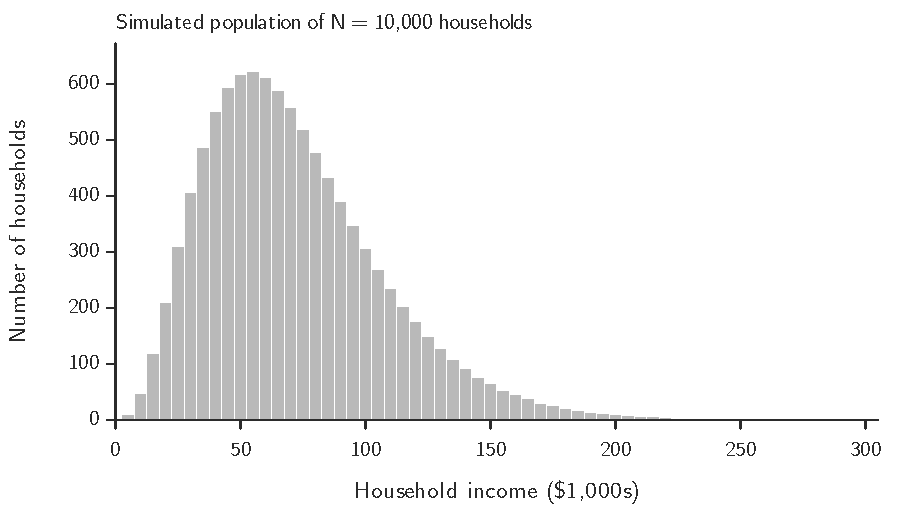
\includegraphics[height=0.62\textheight]{income_pop.pdf}
\end{center}
Let $\mu= \frac{1}{N} \sum_{i=1}^N y_i$ be the population mean and $\sigma^2=\frac{1}{N} \sum_{i=1}^N(y_i-\mu)^2$ the population variance.
}


\frame[t]{
\frametitle{Defining the Estimand}
\scriptsize
% invisible copy of the previous slide's opening line, sized and spaced as
% there (\leavevmode makes it a real paragraph, so it gets \parskip too), so
% the figure sits at exactly the same height on both slides (keep in sync if
% that line changes)
\leavevmode\phantom{Assume a population of $N$ units indexed by $i$ with incomes $y_1,y_2,\dots,y_N$ (fixed numbers).}
\begin{center}
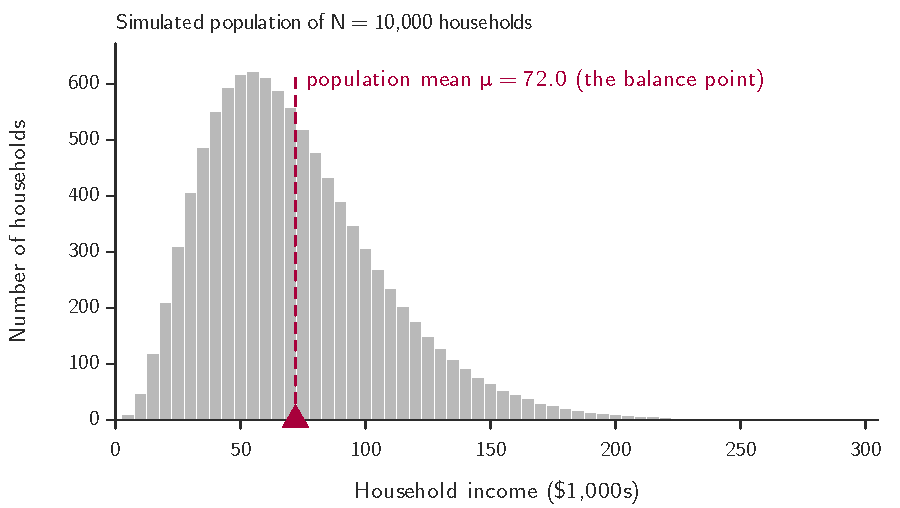
\includegraphics[height=0.62\textheight]{income_pop_mean.pdf}
\end{center}
\normalsize
Let's consider the problem of using sample data from this population to learn about its mean
(i.e. the \alert{true mean}), $\mu$.
}

\frame{
\frametitle{Using Random Samples to Estimate Population Parameters}
\small
Let's look at possible estimators $\widehat{\mu}$ for the (unobserved) mean income in the population $\mu$.\\
\medskip

How can we use sample data to estimate $\mu$? \\
\pause
\bigskip

If we think of a sample of size $n$ as \alert{randomly sampled} with replacement from the population, then $Y_1, \dots ,Y_n$ are \alert{independently and identically distributed} (i.i.d.) random variables with
$E[Y_i] = \mu$ and $V[Y_i] = \sigma^2$ for all $i \in \{1,...,n\}$ (each $Y_i$ is one of $y_1,\dots,y_N$, picked at random).

\pause
\bigskip

In R, we can draw an i.i.d. random sample of size {\tt n} from {\tt population} using
\begin{center}
\texttt{sample(population, size=n, replace=TRUE)}
\end{center}
where \texttt{population} is a vector that contains the $y_i$ values for all $N$ units in the population.
\pause
\medskip

Our estimators, $\widehat{\mu}$, are functions of $Y_1, \dots ,Y_n$ and will therefore be random variables with their own probability distributions. \\

}

\frame{
\frametitle{Income Example: Estimators for the Population Mean}


Candidate estimators:\bigskip
\begin{enumerate}
\item $\widehat{\mu}_1=Y_1$ (the first data observation)\smallskip
\item $\widehat{\mu}_2=4$ (April, the first full month of the baseball season) \smallskip
\item $\widehat{\mu}_3=\overline{Y}_n \equiv \frac{1}{n}(Y_1+ \dots + Y_n)$  (the sample average)
\item $\widehat{\mu}_4=\widetilde{Y}_n \equiv \frac{1}{n+5}(Y_1+ \dots + Y_n)$ (an ``adjusted'' sample average)
\smallskip
\end{enumerate}
\bigskip

How do we choose between these estimators?\\\bigskip

}


%\frame{
%\frametitle{Why the balance point?}
%\begin{itemize}
%\item It is a reasonable measure for the ``center'' of the density.
%\item We have some intuition about balance points.
%\item The balance point tells us a lot about the normal density.
%\item Many intuitive estimators for the density balance point have properties that are easy to describe.
%\end{itemize}
%}

\frame{
\frametitle{Properties of Estimators}

\small
Estimators are random variables, for which randomness comes from \alert{repeated sampling} from the population.

\smallskip

The distribution of an estimator due to repeated sampling is called the \alert{sampling distribution}.

\smallskip

The properties of an estimator refer to the characteristics of its sampling distribution.

\bigskip
\pause

Finite-sample Properties (apply for any sample size):
\begin{itemize}
\item \alert{Unbiasedness}: Is the sampling distribution of our estimator centered at the true parameter value? $E[\hat{\theta}]=\theta$
\item \alert{Efficiency}: Among unbiased estimators, which has the smaller variance? $V[\hat{\theta}_A]< V[\hat{\theta}_B]$\pause
\end{itemize}

Asymptotic Properties (kick in when $n$ is large):
\begin{itemize}
\item \alert{Consistency}: As our sample size grows to infinity, does the sampling distribution of our estimator converge to the true parameter value?
\item \alert{Asymptotic Normality}: As our sample size grows large, does the sampling distribution of our estimator approach a normal distribution?
    %$P(|\hat{\mu_n}-\mu|>\varepsilon)\rightarrow0$ as $n \rightarrow \infty$
%\item Many intuitive estimators for the density balance point have properties that are easy to describe.
\end{itemize}
}


\frame{
\frametitle{Evaluating Sampling Distributions}
\small
Two ways to evaluate the sampling distributions of estimators: \pause
\begin{enumerate}
\item Analytic:
\begin{itemize}
  \item Use formal rules of mathematics and probability to derive properties
  \item Guaranteed to be correct, no ambiguity (unless you screw up the math!)
  \item Might be complicated or even infeasible
\end{itemize}
\pause
\item Simulation:
\begin{itemize}
  \item Do ``repeated experiments'' on your computer
  \item Never exactly correct (cannot repeat $\infty$ times)
  \item Only works for specific scenarios (e.g. you have to assume a specific population)
  \item Easy to implement and often precise enough
\end{itemize}
\end{enumerate}

\pause
\bigskip

Both should yield essentially the same result.

\smallskip

Use one as a check on the other.

}


\frame{
\frametitle{Simulating Sampling Distributions}
\small
Let's simulate the sampling distribution of our four candidate estimators for the population mean:\begin{enumerate}
\item $\widehat{\mu}_1=Y_1$
\item $\widehat{\mu}_2=4$
\item $\widehat{\mu}_3=\overline{Y}_n \equiv \frac{1}{n}(Y_1+ \dots + Y_n)$
\item $\widehat{\mu}_4=\widetilde{Y}_n \equiv \frac{1}{n+5}(Y_1+ \dots + Y_n)$
\end{enumerate}
\bigskip
Algorithm to simulate the sampling distribution of $\widehat{\mu}$
\begin{enumerate}
\item Randomly sample $m$ datasets of size $n$ with replacement from the population:
%\begin{center}
%	\texttt{replicate(m, sample(population, size=n, replace=TRUE))}
%\end{center}
($m$ should be large, choose $n$ as desired)
\item Code a function that implements the estimator and use it to calculate the estimate $\widehat{\mu}$ for each sampled dataset
\item Plot the distribution of estimates $\widehat{\mu}$ with a histogram
\end{enumerate}

}

\begin{frame}[fragile]
  \frametitle{Simulating Sampling Distributions}
  \scriptsize
\begin{Verbatim}[frame=single, label=R Code]
> # population: simulated incomes of 10,000 households ($1,000s)
> length(incomes)
[1] 10000
> incomes[1:30]
 [1]  71.4 125.3  38.2 108.8  53.7  65.0  49.0  66.8  95.8  90.4  51.6
[12] 159.9  90.6  45.4  52.8 115.2  63.6  49.2  46.3 108.1  52.8  66.0
[23]  49.0 115.8  50.5  37.4  33.2  24.7  85.3  62.7
> set.seed(2026)
> # take one random sample
> income.sample <- sample(x=incomes, size=20, replace=TRUE)
> income.sample
 [1]  46.5  35.5 123.1  29.7  67.9  91.2 103.6  40.4 106.1  25.3 129.0
[12]  85.8  66.6  32.0 143.0  63.9  54.0 140.9  12.8  57.9
> # estimator for sample mean
> mean.estimator <- function(x){
+   out <- sum(x)/length(x)
+   return(out)
+ }
> # apply estimator to sample
> mean.estimator(income.sample)
[1] 72.76
\end{Verbatim}
\end{frame}


\begin{frame}[fragile]
  \frametitle{Simulating Sampling Distributions: For Loop}
  \scriptsize
\begin{Verbatim}[frame=single, label=R Code]
> # set parameters
> m <- 100000; n <- 20
> # set up storage matrix for means
> store.means <- matrix(NA, m, 1)
> store.means[1:6, 1]
[1] NA NA NA NA NA NA
> # simulation starts here
> for(i in 1:m){
+   income.sample <- sample(x=incomes, size=n, replace=TRUE)
+   store.means[i, 1] <- mean.estimator(income.sample)
+ }
> store.means[1:6]
[1] 67.315 68.875 70.730 81.975 69.175 66.700
> hist(store.means)
\end{Verbatim}
\end{frame}

\begin{frame}[fragile]
  \frametitle{Simulating Sampling Distributions: Using Matrix Functions}
  \scriptsize
\begin{Verbatim}[frame=single, label=R Code]
> # take m samples of size n
> income.samples <- replicate(m,
+                             sample(x=incomes, size=n, replace=TRUE)
+                             )
> dim(income.samples)
[1]     20 100000
> income.samples[1:3, 1:4]
      [,1]  [,2]  [,3] [,4]
[1,] 132.6 147.9 123.2 41.7
[2,]  18.1  77.9  17.4 52.8
[3,]  98.0  30.8  97.4 37.5
> # compute estimator for each sample
> store.means <- apply(income.samples, 2, mean.estimator)
> store.means[1:6]
[1] 67.495 76.795 63.770 69.725 69.620 80.045
\end{Verbatim}
\end{frame}

\frame{
\frametitle{Sampling Distributions ($m=100{,}000$; $n=20$)}
\vspace{-.35cm}
\begin{figure}[ht] \centering
        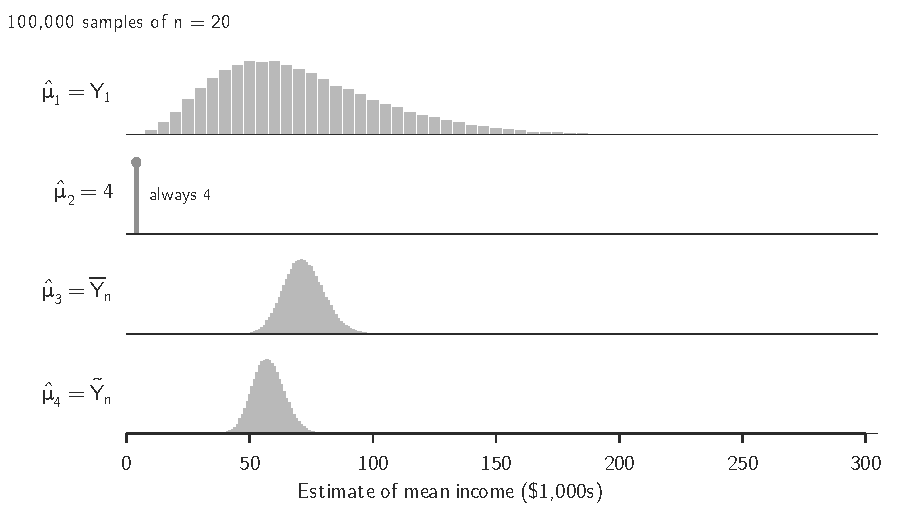
\includegraphics[height=0.82\textheight]{samdist_n20.pdf}
\end{figure}
}


\section{Finite-sample Properties of Estimators}

\subsection{Unbiasedness}

\frame{
\frametitle{Bias}
\small
\begin{definition}[Bias]
\alert{Bias} is the expected difference between an \alert{estimator} $\hat{\theta}$ and a \alert{parameter} $\theta$:
\begin{eqnarray*}
Bias(\hat{\theta}) &=& E\left[\hat{\theta} - \theta  \right] = E\left[\hat{\theta}\right] - \theta
\end{eqnarray*}
\end{definition}
Note that bias is {\bf not} the difference between an estimate ($=$ a particular realized value of an estimator) and a parameter.

\medskip
\pause

\begin{definition}[Unbiasedness]
An estimator is \alert{unbiased} iff:
$$
Bias(\hat{\theta}) = 0\,\,\, \Longleftrightarrow \,\,\,  E\left[\hat{\theta}\right] = \theta
$$
\end{definition}
To check unbiasedness, we need to compute the expected value of the estimator.

%For example, the sample mean is an unbiased estimator for $\mu$.
%\begin{eqnarray*}
%Bias(\overline{X}_n) &=& E\left[\overline{X}_n -  E[X]  \right] \\
%&=& E\left[\hat{\mu} -  \mu \right] \\
%&=& 0
%\end{eqnarray*}
%\vspace{.3cm}
}

\frame{
\frametitle{Deriving the Expected Values of Estimators}
\small
Our candidate estimators:
\begin{enumerate}
\item $\widehat{\mu}_1=Y_1$
\item $\widehat{\mu}_2=4$
\item $\widehat{\mu}_3=\overline{Y}_n \equiv \frac{1}{n}(Y_1+ \dots + Y_n)$
\item $\widehat{\mu}_4=\widetilde{Y}_n \equiv \frac{1}{n+5}(Y_1+ \dots + Y_n)$
\end{enumerate}
\medskip
\pause

\textbf{Worksheet Q1:} Which of $\hat\mu_{1}, \hat\mu_{2}, \hat\mu_{3}, \hat\mu_{4}$ are unbiased?

}

\frame{
\frametitle{Simulating the Expected Values of Estimators}
\vspace{-.35cm}
\begin{figure}[ht] \centering
        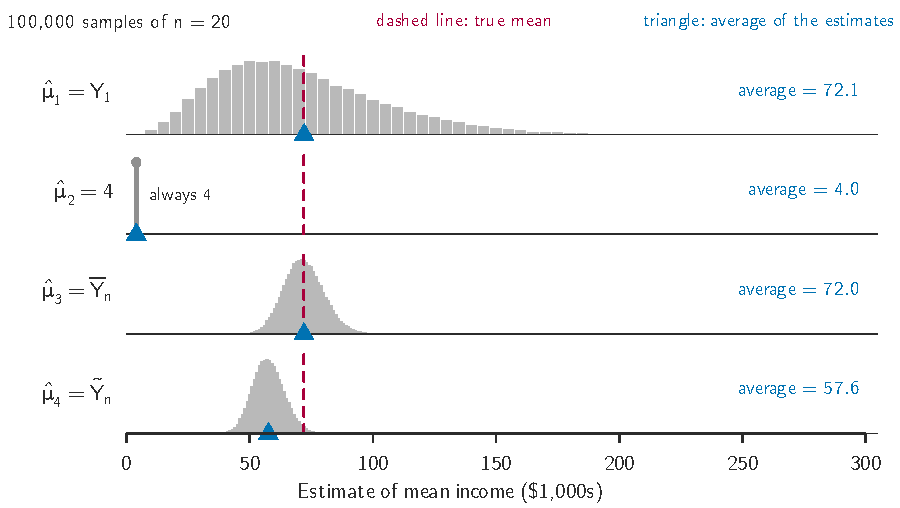
\includegraphics[height=0.82\textheight]{samdist_n20_mean.pdf}
\end{figure}
}

\subsection{Efficiency}

\frame{
\frametitle{Efficiency}
\small
\begin{itemize}
\item How should we choose among unbiased estimators? \pause
\item All else equal, we prefer estimators that have a sampling distribution with smaller variance.
\end{itemize}
\pause
\begin{definition}[Efficiency]
If $\hat{\theta}_A$ and $\hat{\theta}_B$ are two \alert{unbiased} estimators of $\theta$, then $\hat{\theta}_A$ is \alert{more efficient} relative to $\hat{\theta}_B$ iff
$$V[\hat{\theta}_A]< V[\hat{\theta}_B]$$
\end{definition}

\begin{itemize}
    \item Under repeated sampling, estimates based on $\hat{\theta}_A$ are closer to $\theta$ on average (smaller expected squared distance)
    \item Note that this does {\bf not} imply that a particular estimate is always close to the true parameter value
\pause
  \item The standard deviation of the sampling distribution of an estimator, $\sqrt{V[\hat\theta]}$, is often called the \alert{standard error} of the estimator
\end{itemize}

}

\frame{
\frametitle{Deriving the Variances of Estimators}
\small
\vspace{-.5\baselineskip}
\begin{enumerate}
\item $\widehat{\mu}_1=Y_1$
\item $\widehat{\mu}_2=4$
\item $\widehat{\mu}_3=\overline{Y}_n \equiv \frac{1}{n}(Y_1+ \dots + Y_n)$
\item $\widehat{\mu}_4=\widetilde{Y}_n \equiv \frac{1}{n+5}(Y_1+ \dots + Y_n)$
\end{enumerate}\medskip
\textbf{Worksheet Q2:} Derive the variances of $\hat\mu_{1}, \hat\mu_{2}, \hat\mu_{3}, \hat\mu_{4}$. What do you conclude?


% Variances of our candidate estimators: \pause \smallskip
% \begin{enumerate}
% \item $V[\widehat{\mu}_1] = V[Y_1] = \pause \sigma^2$
% \item $V[\widehat{\mu}_2] = V[4] = \pause 0$
% \item $V[\widehat{\mu}_3] = V\left[\frac{1}{n}(Y_1+ \cdots + Y_n)\right] = \pause \frac{1}{n^2}V[Y_1 + Y_2 + \cdots + Y_n]$ \\
% \quad $ = \pause \frac{1}{n^2}(V[Y_1]+V[Y_2]+ \cdots + V[Y_n] + 2Cov[Y_1,Y_2] + \cdots ) $ \\
% \quad $ = \pause \frac{1}{n^2}(V[Y_1]+ \cdots + V[Y_n]) = \pause
%   \frac{1}{n^2}(\sigma^2+\sigma^2+...+\sigma^2) = \frac{1}{n^2}n\sigma^2 = \frac{1}{n}\sigma^2$
% \item $V[\widehat{\mu}_4] = V\left[\frac{1}{n+5}(Y_1+ \cdots + Y_n)\right] = \frac{1}{(n+5)^2}V[Y_1 + Y_2 + \cdots + Y_n]$ \\
% \quad $ = \pause \frac{1}{(n+5)^2}(V[Y_1]+ \cdots + V[Y_n]) = \pause
%   \frac{1}{(n+5)^2}(\sigma^2+\sigma^2+...+\sigma^2) = \frac{n}{(n+5)^2}\sigma^2$
% \end{enumerate}
% \pause
% \medskip
% Between the unbiased estimators (1 and 3), the sample average is more efficient.
}

\frame{
\frametitle{Simulating the Variances of Estimators}
\vspace{-.35cm}
\begin{figure}[ht] \centering
        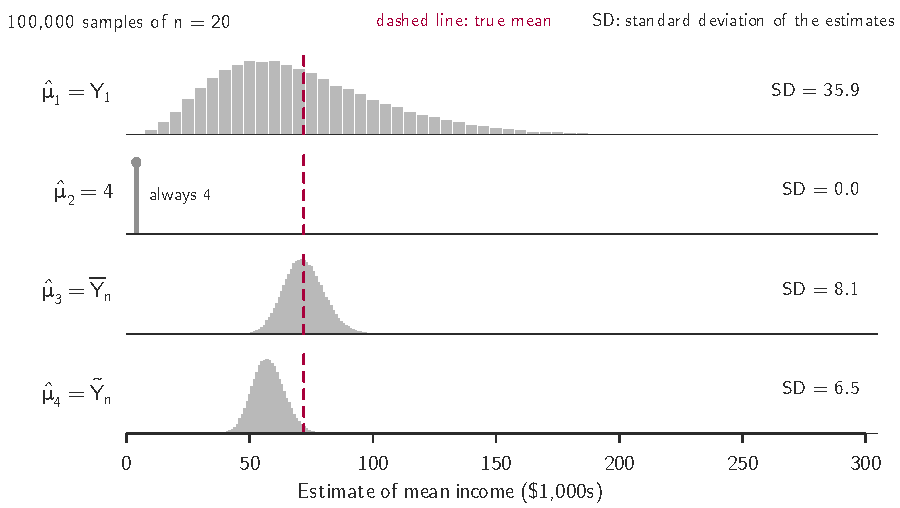
\includegraphics[height=0.82\textheight]{samdist_n20_sd.pdf}
\end{figure}
}

\frame{
\frametitle{Mean Squared Error}
\small
How can we choose between an unbiased estimator and a biased estimator with smaller variance?
\pause
\medskip

\begin{definition}[Mean Squared Error]
To compare estimators in terms of both efficiency and unbiasedness we can use the \alert{Mean Squared Error} (MSE), the expected squared difference between $\hat{\theta}$ and $\theta$:
$$
MSE(\hat{\theta}) = E\left[(\hat{\theta} - \theta)^2\right] = Bias(\hat{\theta})^2 + V(\hat{\theta})
$$
\end{definition}
\pause
\medskip

\textbf{Worksheet Q3--Q4:}
\begin{itemize}
  \item Q3: Prove the decomposition above.
  \item Q4: Show: $MSE(\widehat{\mu}_1)=\sigma^2$, $MSE(\widehat{\mu}_2)=(4-\mu)^2$, $MSE(\widehat{\mu}_3) = \frac{\sigma^2}{n}$, and $MSE(\widehat{\mu}_4) = \frac{25\,\mu^2+n\,\sigma^2}{(n+5)^2}$.
\end{itemize}
}

%\frame{
%\frametitle{Example}
%
%Assume an $i.i.d.$ sample and recall the two possible definitions of sample variance:
%
%\begin{displaymath}
%S_{0_n}^2 = \frac{1}{n}\sum_{i=1}^n (X_i-\overline{X}_n)^2
%\end{displaymath}
%\begin{displaymath}
%S_{1_n}^2 = \frac{1}{n-1}\sum_{i=1}^n (X_i-\overline{X}_n)^2
%\end{displaymath}
%
%\vspace{.3cm}
%
%Which has less bias? \\
%
%\vspace{.3cm}
%
%Which has smaller variance?  \\
%
%\vspace{.3cm}
%
%Which has smaller MSE?
%
%}

\section{Asymptotic Properties of Estimators}

\subsection{Consistency}

\frame{
\frametitle{Asymptotic Evaluations}

\begin{itemize}
  \item Unbiasedness and efficiency are \alert{finite-sample properties} of estimators,
  which hold regardless of sample size
  \item Estimators also have \alert{asymptotic properties}, i.e., the characteristics of
  sampling distributions when sample size becomes infinitely large
\pause
\medskip
  \item To define asymptotic properties, consider a \alert{sequence} of estimators at increasing sample sizes:
  $$\hat\theta_1, \hat\theta_2, ..., \hat\theta_n$$
  \item For example, for i.i.d. draws $X_1, X_2, \dots$ (such as the incomes $Y_i$), the sequence of sample means ($\bar{X}_n$) is defined as:
  $$ \bar{X}_1, \bar{X}_2, ..., \bar{X}_n \ = \ X_1, \frac{X_1+X_2}{2}, ..., \frac{X_1 + \cdots + X_n}{n} $$
\pause\vspace{-1em}
  \item Asymptotic properties of an estimator are defined by the behavior of $\hat\theta_1,...\hat\theta_n$ when $n$ goes to infinity.
\end{itemize}
}

\frame{
\frametitle{Stochastic Convergence}
\begin{itemize}
 \item When a sequence of random variables stabilizes to a certain probabilistic behavior as $n\to\infty$, the sequence is said to show \alert{stochastic convergence}.

\pause
\bigskip

 \item Two types of stochastic convergence are of particular importance:

  \begin{enumerate}
    \item \alert{Convergence in probability}: the probability of an ``unusual'' value becomes increasingly smaller as the sequence progresses such that values eventually stabilize in taking on a constant value\\
    (i.e. the \alert{limiting distribution} is a constant)\medskip
    \item \alert{Convergence in distribution}: values in the sequence continue to vary, but the variation eventually comes to follow an unchanging distribution as the sequence progresses \\
    (i.e. the limiting distribution is a well characterized distribution)
  \end{enumerate}

\end{itemize}
}


\frame{
\frametitle{Convergence in Probability}
\small
\vspace{-.25\baselineskip}
\begin{definition}[Convergence in Probability]
A sequence $W_1, W_2, \dots$ of random variables \alert{converges in probability} towards a real number $a$ if, for all accuracy levels $\varepsilon > 0$,
$$
\lim_{n\to\infty}\Pr\big(|W_n-a| \geq \varepsilon\big) = 0 $$
We write this as
$$ W_n \ \xrightarrow{p}\ a \quad \mbox{ or } \quad
\underset{n\to\infty}{\operatorname{plim}}\, W_n = a. $$
\end{definition}
\begin{itemize}
\item As $n$ increases, almost all of the PDF of $W_n$ will be concentrated in the $\varepsilon$-interval around $a$, $[a-\varepsilon,a+\varepsilon]$
%\item It remains possibility that $|X_n -a| > \varepsilon$ but this is becomes increasingly infrequenthappens an infinite number of times, although at infrequent intervals.

\pause

  \item A sufficient condition for convergence in probability:
 $$E[W_n]\rightarrow a \quad \text{and} \quad V[W_n]\rightarrow 0 \quad \text{as} \quad n\to\infty $$
\pause
\vspace{-1.25\baselineskip}
 \item For example, if the $X_i$ are i.i.d. with finite variance $\sigma^2$, the sample mean $\bar{X}_n$ converges to the population mean $\mu$ in probability because
\vspace{-.25\baselineskip}
 $$ E[\bar{X}_n] \rightarrow \mu \quad \text{and} \quad V[\bar{X}_n] = \sigma^2/n \rightarrow 0
 \quad \text{as} \quad n \to \infty $$
% counterexample added 2026-09-28 (a student asked why the condition is not necessary)
\pause
\vspace{-1.25\baselineskip}
 \item The condition is sufficient, not necessary. Take $W_n = n$ with probability $1/n$ and $W_n = 0$ otherwise:
\vspace{-.25\baselineskip}
 $$ \Pr\big(|W_n - 0| \geq \varepsilon\big) \leq 1/n \rightarrow 0, \text{ so } W_n \xrightarrow{p} 0, \quad \text{but} \quad
 E[W_n] = 1 \quad \text{and} \quad V[W_n] = n - 1 \rightarrow \infty $$

\end{itemize}

}

\frame{
\frametitle{Sample Mean Converges to Population Mean in Probability}
\begin{center}
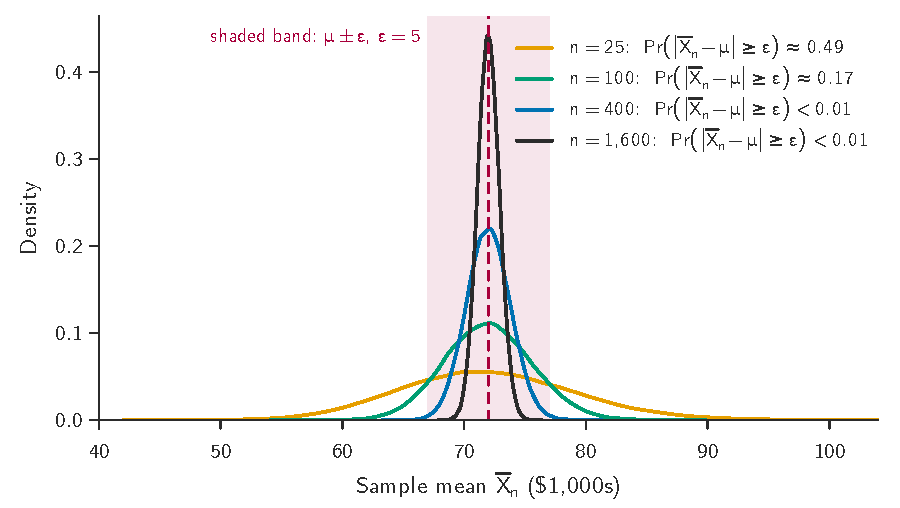
\includegraphics[height=0.82\textheight]{mean_concentration.pdf}
\end{center}

}



\frame{
\frametitle{Consistency}
\small
\begin{definition}
An estimator $\hat\theta_n$ is \alert{consistent} if the sequence $\hat\theta_1, ..., \hat\theta_n$
converges in probability to the true parameter value $\theta$ as the sample size $n$ grows to
infinity:
$$\hat\theta_n\xrightarrow{p} \theta \quad \text{or} \quad
\underset{n\to\infty}{\operatorname{plim}}\, \hat\theta_n = \theta $$
\end{definition}
\pause
\begin{itemize}
  \item Often seen as a minimal requirement for estimators
  \item A consistent estimator may still perform badly in small samples
\pause
\medskip
  \item Two ways to verify consistency:
  	\begin{enumerate}
	 \item Analytic: Often easier to check if $E[\hat\theta_n] \to \theta$ and $V[\hat\theta_n]\to 0$
	 \item Simulation: Increase $n$ and see how the sampling distribution changes
	\end{enumerate}
\pause
\medskip
   \item Does unbiasedness imply consistency?
   \item Does consistency imply unbiasedness?
\end{itemize}

}



\frame{
\frametitle{Deriving Consistency of Estimators}

Our candidate estimators:
\begin{enumerate}
\item $\widehat{\mu}_1=Y_1$
\item $\widehat{\mu}_2=4$
\item $\widehat{\mu}_3=\overline{Y}_n \equiv \frac{1}{n}(Y_1+ \dots + Y_n)$
\item $\widehat{\mu}_4=\widetilde{Y}_n \equiv \frac{1}{n+5}(Y_1+ \dots + Y_n)$
\end{enumerate}\bigskip

Which of these estimators are consistent for $\mu$? (The subscript on $\widehat{\mu}_k$ labels the estimator; each is computed at every sample size $n$.) \pause
\smallskip
\begin{enumerate}
\item $E[\widehat{\mu}_1] = \mu$ and $V[\widehat{\mu}_1] =\sigma^2$
\item $E[\widehat{\mu}_2] = 4$ and $V[\widehat{\mu}_2] = 0$
\item $E[\widehat{\mu}_3] = \mu$ and $V[\widehat{\mu}_3] = \frac{1}{n}\sigma^2$
\item $E[\widehat{\mu}_4] = \frac{n}{n+5}\mu$ and $V[\widehat{\mu}_4] = \frac{n}{(n+5)^2}\sigma^2$
\end{enumerate}


}

% The next three frames are one run: same figure size and position.
\frame[t]{
\frametitle{Sampling Distributions of Estimators ($n=20$)}
\scriptsize
{\centering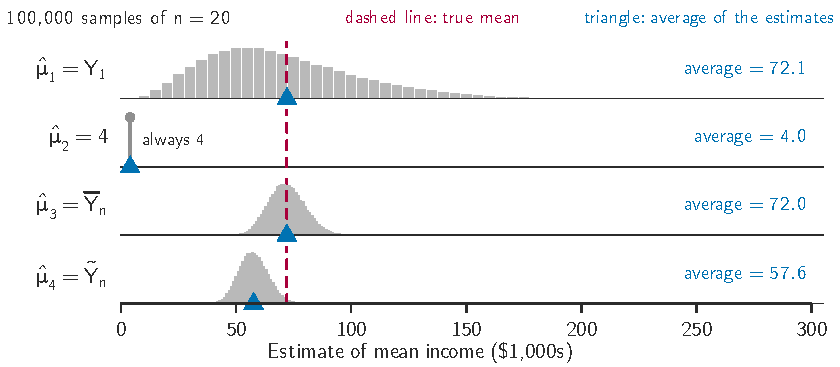
\includegraphics[height=0.66\textheight]{consist_n20.pdf}\par}
}

\frame[t]{
\frametitle{Sampling Distributions of Estimators ($n=100$)}
\scriptsize
{\centering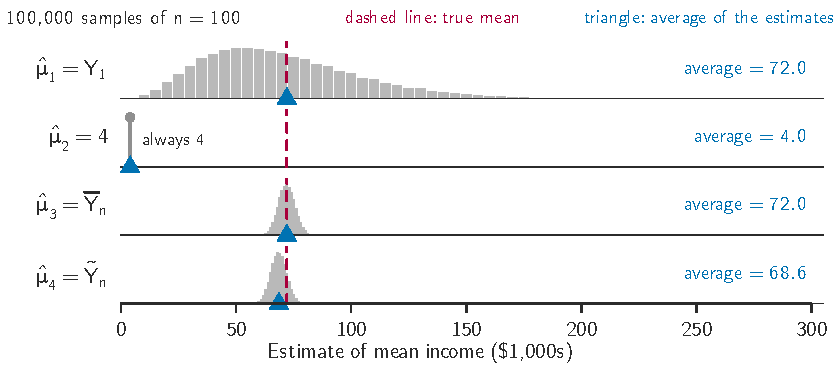
\includegraphics[height=0.66\textheight]{consist_n100.pdf}\par}
}

\frame[t]{
\frametitle{Sampling Distributions of Estimators ($n=3000$)}
\scriptsize
{\centering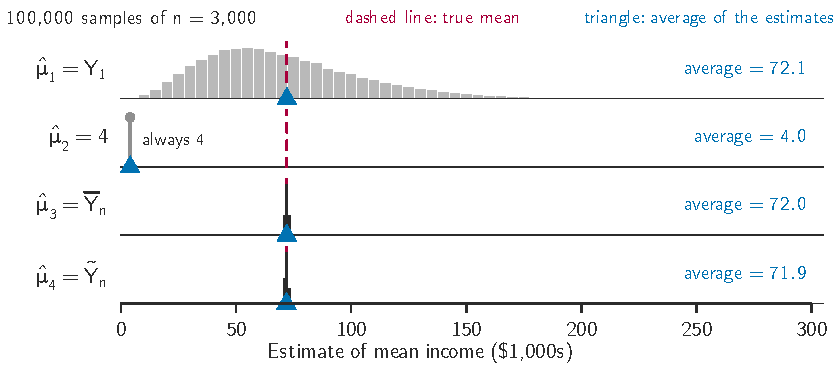
\includegraphics[height=0.66\textheight]{consist_n3000.pdf}\par}

\pause
Therefore,
\begin{center}
\begin{tabular}{ll}
$\widehat{\mu}_1$: Unbiased but inconsistent & $\widehat{\mu}_2$: Biased and inconsistent \\
$\widehat{\mu}_3$: Unbiased and consistent & $\widehat{\mu}_4$: Biased but consistent \\
\end{tabular}
\end{center}

}

\frame[t]{
\frametitle{Weak Law of Large Numbers}
\small
\begin{theorem}[Weak Law of Large Numbers]
Let $X_1, X_2, \dots, X_n$ be a sequence of i.i.d. random variables, each with finite mean $\mu$. Then for all $\varepsilon>0$,
$$ \overline{X}_n\ \xrightarrow{p}\ \mu \quad \mbox{as} \quad n \to \infty $$
or equivalently,
$$  \lim_{n\to\infty}\Pr\!\left(\,|\overline{X}_n-\mu| \geq \varepsilon\,\right) \ = \ 0$$
where $\overline{X}_n$ is the sample mean.
\end{theorem}
\begin{itemize}
\item LLN says that the sample average converges in probability to the (common) expected value $\mu$ as the sample size grows large.
\item In other words, the sample mean is a consistent estimator \alert{for any population distribution with a finite mean}.
\end{itemize}
}


\frame[t]{
\frametitle{Example: Mean of $n$ independent tosses of a coin
}

\begin{figure}[ht] \centering
        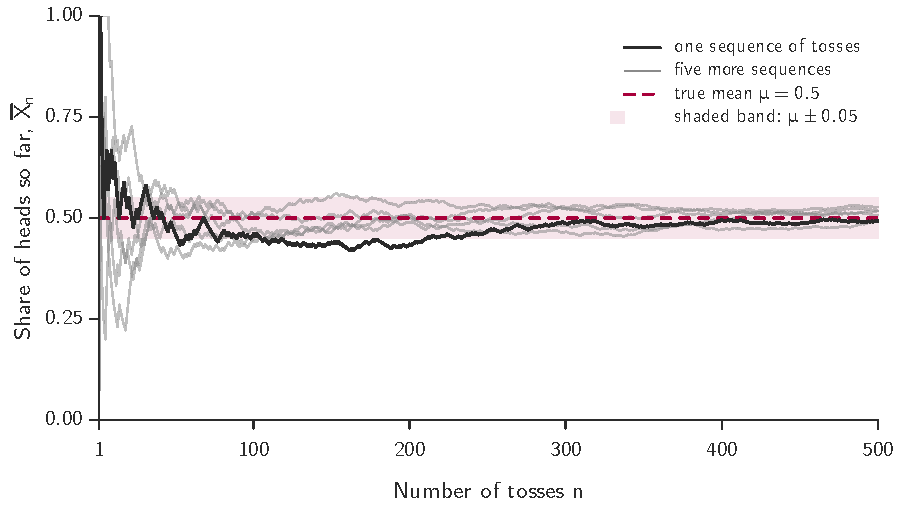
\includegraphics[height=0.82\textheight]{lln_coin.pdf}
\end{figure}
}

\subsection{Asymptotic Normality}



\frame{
\frametitle{Asymptotic Distributions of Estimators}
\begin{itemize}
\addtolength{\itemsep}{.25\baselineskip}
\item In reality, the sample size never equals infinity.
\item Therefore, an estimator has a \alert{non-degenerate} (i.e. non-zero variance)
sampling distribution in practical situations.
\item It would be useful to know something about this distribution when the sample size is large but not infinite.
\medskip
\pause
\item How can we study the properties of large, but not infinitely large, samples?
\item It turns out that we can use asymptotic theory to \alert{approximate} the sampling
distributions of estimators from finite large samples.
\item Such approximated distributions are called the \alert{asymptotic distributions} of
estimators.
\end{itemize}
}



\frame{
\frametitle{Convergence in Distribution}
\small
\begin{Definition}[Convergence in Distribution]
Consider a sequence of random variables $W_1, W_2, \dots$, each with CDFs $F_1, F_2, \dots$.
The sequence is said to \alert{converge in distribution} to a limiting random variable $W$ with
CDF $F$ if
$$
    \lim_{n\to\infty} F_n(x) = F(x),
$$
for every point $x$ at which $F$ is continuous.  We write this as
$$ W_n \ \stackrel{d}{\rightarrow} \ W. $$
\end{Definition}

\begin{itemize}
   \item As $n$ grows, the distribution of $W_n$ converges to the distribution of $W$.
   \item Convergence in probability is a special case of convergence in distribution in which the distribution converges to a \alert{degenerate distribution} (i.e. a probability distribution which only takes a single value).
\end{itemize}

}


\frame{
\frametitle{Limit Distribution of the $\sqrt{n}$-scaled Sample Mean}
\small
\begin{itemize}
  \item Consider the random variable $\overline{X}_n - \mu$, the fluctuation
  of the sample mean around the population mean.
  \item What does this converge to? \pause By LLN, $\overline{X}_n - \mu \ \xrightarrow{p} \ \mu - \mu = 0$. \\ \pause
  It converges to a degenerate distribution because
  $$V[\overline{X}_n - \mu] = \sigma^2 / \alert{n} \to 0 \quad \text{as} \quad n\to\infty.$$
  \pause
  \item Now, consider $\sqrt{n}(\overline{X}_n - \mu)$, the fluctuation {\bf scaled}
  by the factor of $\sqrt{n}$.
  \item Does this converge to a degenerate distribution? \pause Its variance stays at $\sigma^2$ for every $n$:
  $$V[\sqrt{n}(\overline{X}_n - \mu)] = \alert{n} \cdot \sigma^2 / \alert{n} = \sigma^2.$$
  (we carefully choose the scale $\sqrt{n}$ such that the variance neither shrinks
  to $0$ nor blows up to $\infty$.)
  This suggests, and the CLT on the next slide proves, that the limit is not degenerate.
  \pause
  \item Then what non-degenerate distribution does this converge to? It turns out...
\end{itemize}
}

\frame{
\frametitle{Central Limit Theorem}
\begin{theorem}[Lindeberg--L\'evy Central Limit Theorem]
Let $X_1, ...,X_n$ be a sequence of i.i.d. random variables each with mean $\mu$ and variance $\sigma^2 < \infty$. Then, for \alert{{\it any}} population distribution of $X$,
$$ \sqrt{n}(\overline{X}_n - \mu) \ \xrightarrow{d} \ \cN(0, \sigma^2 ).$$
\end{theorem}
\begin{itemize}
\item As $n$ grows, the distribution of the difference between the sample mean and its limit $\mu$, when scaled by $\sqrt{n}$, converges to a normal distribution with mean 0 and variance $\sigma^2$.
\pause
\item CLT also implies that the \alert{standardized} sample mean converges to a
standard normal random variable:
$$ Z_n \ \equiv \ \frac{\overline{X}_n - E\l[\overline{X}_n\r]}{\sqrt{V\l[\overline{X}_n\r]}}
\ = \ \frac{\overline{X}_n - \mu}{\sigma/\sqrt{n}}
\ \xrightarrow{d} \ \cN(0,1). $$
\item Note that CLT holds for a random sample from {\it any} population distribution with finite variance --- what a convenient result!
\end{itemize}

}

\frame{
\frametitle{Central Limit Theorem}

\begin{figure}[ht] \centering
        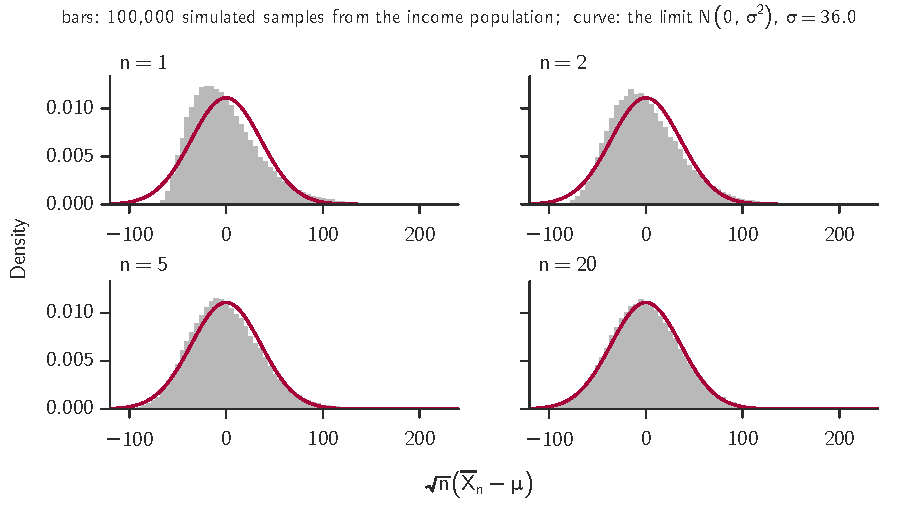
\includegraphics[height=0.82\textheight]{clt_scaled_mean.pdf}
\end{figure}

}


\frame{
\frametitle{Asymptotic Normality}
\begin{itemize}
 \item Now let's consider estimators from a large, but not infinitely large, sample.
 \item CLT implies that, for a sufficiently large sample, we have:
 $$ \frac{\overline{X}_n - \mu}{\sigma/\sqrt{n}} \ \stackrel{\text{approx.}}{\sim} \ \cN(0,1)$$
 \item This implies:
 $$ \overline{X}_n \ \stackrel{\text{approx.}}{\sim} \ \cN\l(\mu, \frac{\sigma^2}{n}\r)$$
 \item That is, the (unstandardized) sample mean itself is also approximately normally
 distributed when sample size is large.
 \item An estimator is \alert{asymptotically normal} if its asymptotic distribution is normal.
\end{itemize}
}


\frame{
\frametitle{Verifying Asymptotic Normality by Simulation}
\vspace{-.35cm}
\begin{figure}[ht] \centering
        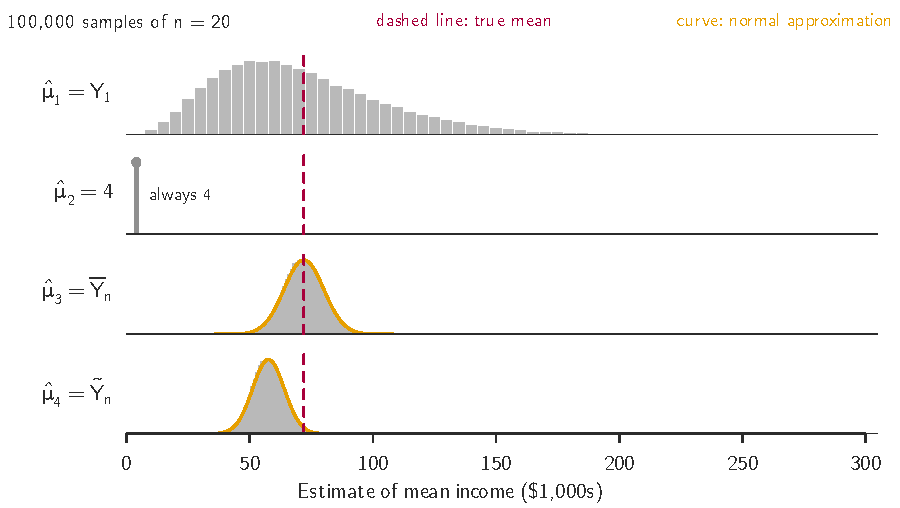
\includegraphics[height=0.82\textheight]{samdist_n20_normal.pdf}
\end{figure}

}

\frame{
\frametitle{Summary}
\small
\begin{tabular}{c|c|c}
  Concept & Criteria & Intuition \\
  \hline
  & & \\
  Unbiasedness & $E[\hat{\mu}]=\mu$ & Right on average \\
  & \\
  Efficiency & $V[\hat{\theta}_A]< V[\hat{\theta}_B]$ & Lower variance (among unbiased estimators) \\
  & \\
  Consistency & $\hat{\mu}_n\stackrel{p}{\rightarrow}\mu$ & Converge to estimand as $\ n \to \infty$ \\
  & \\
  Asymptotic Normality & $\overline{X}_n \stackrel{\text{approx.}}{\sim} \cN(\mu,\frac{\sigma^2}{n})$ & Approximately normal in large $n$ (sample mean shown) \\

\end{tabular}


}

\frame{
\frametitle{Analogy Principle}
\small
\begin{Definition}
The \alert{analogy principle} tells us to estimate a characteristic in
the population using the same characteristic in the sample.
\end{Definition}\vspace{-.1in}\pause
\begin{itemize}
\item For example, following the analogy principle, we estimate the population
mean $\mu_Y$ using the sample mean $\bar{Y}$:
\[
\bar{Y}=\frac{1}{n}\sum_{i=1}^n Y_i.
\] \pause
%\item Note that the sample mean is a function of the sample (it gives us
%a value for $\bar{Y}$, an estimate, for each particular sample.)
\item To estimate $\sigma^2_Y$, the analogy principle gives the \alert{plug-in} estimator, which divides by $n$ as the definition of $\sigma^2$ does:
\[
\widehat{\sigma}^2_Y =\frac{1}{n}\sum_{i=1}^n (Y_i-\bar{Y})^2.
\]
(Lecture 2-2: dividing by $n-1$ instead gives the unbiased \alert{sample variance} $S_n^2$.)
  \item As the sample size increases and the sample ``approaches'' the population
we expect sample characteristic to converge to the population characteristics.
\end{itemize}

}


\end{document}
